\chapter{Machine learning approach for true track tagging}
Applying cuts to track features in order to differentiate between improved the ratio of true and false reconstructed tracks, slightly. A more effective
approach in classifying a track as true or false can be achieved with a machine learning algorithm for classification. Unlike one dimensional cuts, a machine learning
algorithm can be implemented to find correlations between the input feature for a more accurate identification of true tracks. The library used for
machine learning is XGBoost, which is explained in the following section.

\section{XGBoost}
XGBoost \cite{xgboost} is a gradient boosting machine learning algorithm, which primarily uses decision trees as a predictive model for classification and regession analysis.
It is used for supervised learning problems to predict a target variable $y_i$ based on the training data $x_i$ containing multiple features. The model
of XGBoost describes the mathematical structure, which determines the prediction from its input data. A linear model is a common example, where the predictions
are linear combinations of the weighted input features:
\begin{align}
  \hat{y}_i = \sum_j \Theta_j x_{ij}
\end{align}
The coefficents $\Theta$ are indefinite parameters that need to be learned from the training data. Thus, the task of training is in determining the optimal parameters
for the target variable $y_i$ based on our input $x_i$. In order to train a model, an objective function needs to be defined, which measures how well
the model fits the training data. Those functions consist of the training loss function $L(\Theta) $ and the regularization term $\Omega (\Theta)$.
\begin{align}
  \text{obj}(\Theta) = L(\Theta) + \Omega(\Theta)
\end{align}

The training loss function is commonly defined as the mean squared error or logistic loss for logisitc regression problems:
\begin{align}
  &L(\Theta) = \sum_i (y_i - \hat{y}_i)^2 \\
  &L(\Theta) = \sum_i [y_i \ln{(1 + e^{-\hat{y}_i})} + (1 - y_i) \ln{(1 + e^{-\hat{y}_i})}]
\end{align}
The regularization term describes the complexity of a model in order to prevent overfitting.

\section{Decision tree ensemble}
The model used by the XGBoost library is the decision tree ensemble, which consists of a set of classification and regression tress (CART).
A CART assigns a prediction score to each of the leaves in which the input features are classified. The prediction of a single tree is usually not accurate,
therefore the prediction of numerous trees is summed together. This method can be written mathematically as:
\begin{align}
  &\hat{y}_i = \sum_{k=1}^K f_k(x_i)\,, \: f_k \in \mathcal{F} \\
  &\text{obj}(\Theta) = \sum_i^n l(y_i, \hat{y}_i) + \sum_{k=1}^K \Omega(f_k)
\end{align}
Where $K$ is the number of trees, $\mathcal{F}$ the set of all possible CARTs and $f$ a function in $\mathcal{F}$. A decision tree ensemble is shown exemplary in
figure \ref{fig:random_forest}.

\begin{figure}
  \centering
  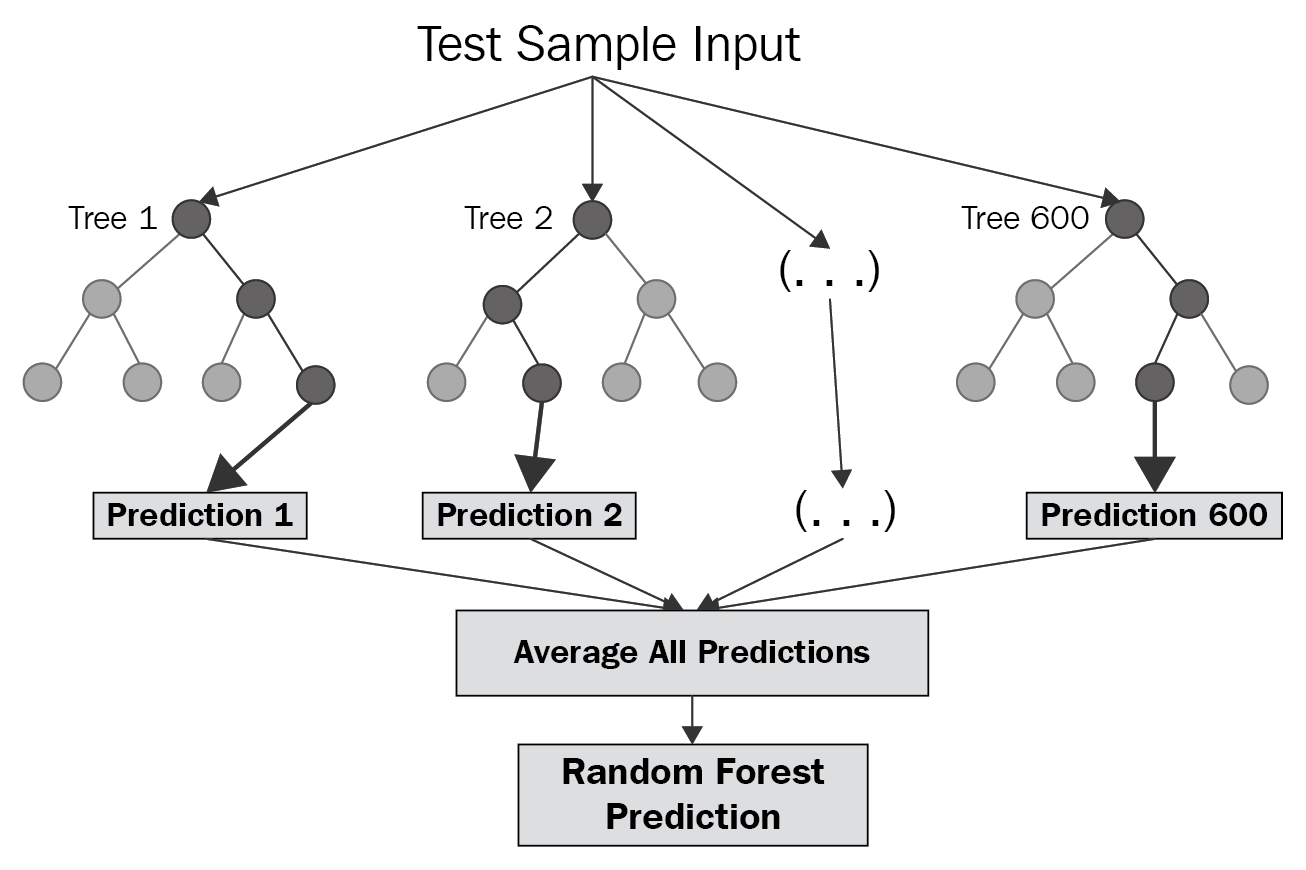
\includegraphics[height=0.6\textwidth]{images/random_forest.png}
  \caption{Representation of a decision tree ensemble \cite{random_forest}.}
  \label{fig:random_forest}
\end{figure}

\section{Boosted trees}
The model used for boosted trees and a random forest is both the tree ensembles with the only difference being the training method. Optimizing the objective functions for
boosted trees is achieved by additive training. This means that everything learned is fixed and only one new tree per step $t$ is added. This can be written
down as follows:
\begin{align}
  \hat{y}_i^{(t)} = \sum_{k=1}^t f_k(x_i) = \hat{y}_i + f_t(x_i)
\end{align}

The tree added in each step is supposed to optimize our objective. For a mean squared error loss function, the objective at step $t$ can be written as:
\begin{align}
  \text{obj}^{(t)} &= \sum_{i=1}^n \left[g_i f_t(x_i)] + \frac{1}{2}h_i f_t^2(x_i)\right] + \Omega(f_t)  \\
  g_i &= \partial_{\hat{y}_i^{(t-1)}} l(y_i, \hat{y}_i^{(t-1)}) \\
  h_i &= \partial^2_{\hat{y}_i^{(t-1)}} l(y_i, \hat{y}_i^{(t-1)})
\end{align}

The value of the objective function only depends on $g_i$ and $h_i$, giving XGBoost the advantage of using custom loss functions including logistic regression.

However, the regularization term still needs to be defined. One definition that works well in practice and thus used by XGBoost is:
\begin{align}
  \Omega (f) = \gamma T + \frac{1}{2}\lambda \sum_{j=1}^T \omega_j^2
\end{align}
Here, $\omega_{q(x)}$ is the vector of scores on leaves, $q$ is a function that assigns each data point to the corresponding leave and $T$ is the number of leaves.

With this definition, the objective function can be compressed to:
\begin{equation} \label{eqn:obj}
  \text{obj} = -\frac{1}{2}\sum_{j=1}^T \frac{G_j^2}{H_j + \lambda} + \gamma T
\end{equation}
Here, $G_j$ and $H_J4$ are the sum over all $g_i$ and $h_i$ repsectively. Equation \ref{eqn:obj} is a measure for how good a structure tree is. Its score
is determined by the statistics $g_i$ and $h_i$ in the leaves, with a smaller score meaning a better tree structure.
Since it is not feasible to enumerate all possible tress to find the best one, only one level of a tree is optimized at a time.
For each split of a leaf into a new left and right leaf, the gained score is defined as:
\begin{equation}
  \text{Gain} = \frac{1}{2}\left[\frac{G_L^2}{H_L + \lambda} + \frac{G_R^2}{H_R + \lambda} - \frac{(G_L + G_R)^2}{H_L+H_R+\lambda}\right] -\gamma
\end{equation}

Optimal splits are then determined by sorting all instances and calculate the structure score of all possible split solutions.

\section{Machine learning setup}
The data used to train the learner %is identical to the one from section \ref{sec:feature} and
consists of 400000 generated $\SI{200}{\mega\eV}$ protons with ten protons per event
traversing the telescope described in section \ref{sec:setup}. The protons
are reconstructed with Corryvreckan, with the true tracks being identified with the MC truth from Allpix$^2$ and masked for the learner. A total number of 92546 tracks
are reconstructed, with 36340 being true tracks.
To test the learner, another simulation, being identical to the one in \ref{sec:feature} is used and consists of 100000 protons with ten protons per event.

The objective of the learner is binary logistic, which performs a logistic regression and outputs a probability for classifying a track as true or false.
Therefore, a logistic loss function is used for training the model.
To determine the optimal number of boosting rounds, early stopping is utilized on a validation set, consisting of 100000 generated protons. This means, that
the model will train until the validation score stops improving for ten consecutive boosting rounds, with the number
of boosting rounds belonging to the highest validation score being chosen for testing. In this case, the validation score refers to the area under the
Receiver Operating Characteristic (ROC) curve. \\
The ROC curve describes the true positive rate $TPR = t_p/(t_p + f_p)$ as a function of the false positive rate $FPR = f_p/(f_p + t_n)$ with
$t_p$, $t_n$ and $f_p$ meaning the true positive, true negative and false positive classification of a track respectively. The larger the area under the curve (auc) in respect
to the diagonal, which represents random classification, the better the performance of the classificator. \\
All features, including $\chi^2$, kink angles, cluster positions and charge depositions are selected as input for the classifier. Less useful features
may not contribute significantly for classification, but also do not disrupt the learning process, as trees do not split as often on variables with little impact.
Thus, no problems will arise by taking all features into account, as long as the training data is sufficiently large to be able to compensate for inefficiencies.

Tuning several hyper parameters is necessary to ensure an optimal performance of the classificator. Taking many hyper parameters and values into account, comes at the
cost of a large computation time. For this reason, four parameters are chosen to be optimised. The maximum depth of each tree influences the
complexity of the model and the likeliness of overfitting. With the learning rate $\eta$, overfitting can be prevented as it represents a weighting factor for
corrections added by new trees in the model. It takes values from zero to one, with smaller values describing smaller corrections from further trees. \\
The minimum loss reduction required for an additional partition on a leaf node is referred to as $\gamma$. A similar impact has the minimum sum of instance weight $\theta$
needed in a child. Leaf nodes with a sum of weights less than the specified value will prevent further tree partition steps.
Both the $\theta$ and $\gamma$ take values from 0 to $\infty$ and are a measure for how conservative the algorithm will be, with larger values representing a more
conservative algorithm.

A grid search from the library Scikit-learn \cite{scikit} is used to determine an optimal value for each of the parameters mentioned above. The values given as input into the grid search
are shown in table \ref{tab:grid}.

  \begin{table}
    \centering
    \begin{tabular}{c c c c}
      \toprule
      tree depth & $\eta$ & $\gamma$ & $\theta$ \\
      \midrule
      3 & 0.05 & 0.5 & 1  \\
      4 & 0.1  & 1   & 25  \\
      5 & 0.3  & 2 & 50  \\
      6 & 0.7  & 5   &  \\
    \end{tabular}
    \caption{Parameter values that are used for the grid search. The tree depth refers to the maximum depth of a tree, $\eta$ refers to the learning rate,
    $\gamma$ is a threshold for the allowed minimum loss reduction in a partition step and $\theta$ is the minimum sum of instance weight needed in a child.}
    \label{tab:grid}
  \end{table}
To quantify each different combination of the hyper parameter values, a 5-fold cross validation is performed. This means that the data set is split into five equally
large sets, with the learner training on four of them and evaluating on the last one. Each of the five sets serves as the test data, which means that for each
parameter combination five runs are performed. The area under the ROC curve serves as the scoring function to measure how good the predicition on the test data set is.
A mean of the five auc values represents the score, which is compared in the grid search. Thus, the cross validation helps to compensate for variability in the simulated
data to derive an accurate estimate of the predictive power of the model. \\
The maximal AUC of $0.579(3)$ is achieved with a maximum tree depth of 5, $\eta=0.7$, $\gamma=5$ and $\theta=25$. With $\gamma=5$, the result of the grid search of the remaining
parameters can be visualized and is shown in figure \ref{fig:grid}

\begin{figure}
  \centering
  \includegraphics[height=0.6\textwidth]{plots/grid_search.pdf}
  \caption{The mean test score referring to the auc for the different hyper parameter configurations with the errorbars being the standard deviation of the mean. The
  smaller bars refer to $\eta$, the larger bars to $\theta$ and the red marked value to the maximal AUC.}
  \label{fig:grid}
\end{figure}

Varying the values of the hyper parameters only causes small changes in the mean test score, especially the learning rate has a negligible influence on the AUC. Taking the
standard deviations into account makes it impossible to determine, wether the best combination of hyper parameters actually have the highest AUC. However, due to the
small differences, no significant impact is to be expected in this case. For that reason, the above mentioned hyper parameter values are chosen for training and testing the model.

\section{Machine learning results}
To compare the performance of the learner on the train and test data, the normalised distribution of the output probabilities are investigated.
These are shown in figure \ref{fig:output} alongside the corresponding differences.

\begin{figure}
  \hspace{-2.5cm}
  %\centering
  \begin{subfigure}{0.62\textwidth}
      \centering
      \includegraphics[height=0.82\textwidth]{plots/output_normed.pdf}
  \end{subfigure}
  \begin{subfigure}{0.62\textwidth}
      %\centering
      \hspace{0.95cm}
      \includegraphics[height=0.82\textwidth]{plots/output_difference.pdf}
  \end{subfigure}
  \caption{Normalised probabilitiy distributions of tracks being true and false for the train and test data set shown on the left.
  The corresponding differences between the performance on the training and testing data is shown on the right.}
  \label{fig:output}
\end{figure}

The distribtions of the train and test data predictions show small differences, indicating that no signifiacnt overtraining occurs during the training process.
%For both true and false tracks, the greatest deviations are found at their most probable value, between 0.8 and 0.9.
Both true and false tracks have a maximum around 0.8 as their most probable value, though the peak for the true tracks is higher due to the larger number
of false tracks assigned to small probabilities of being true. Also noteworthy is, that a neglicable number of tracks have a probability of 0.9 and higher. This means that
with the given input, a lot of false combinations of clusters still show similar properties to true tracks.

The usefullness of the individual features to classify the reconstructed tracks can be quantified with the number of times each feature was split on.
This feature importance score is shown in figure \ref{fig:importance}.

\begin{figure}
  \centering
  \includegraphics[height=0.6\textwidth]{plots/feature_importance_all.pdf}
  \caption{The number of splits of each feature used as input for the learner.}
  \label{fig:importance}
\end{figure}

All three features, which proved to be useful for classifying tracks with cuts have a high feature score, highlighting their importance for separating true and false tracks.
Other features with a high number of splits, like the vertical kink angle of the second plane can still be useful for the learner in combination with other features, even though
their use for classifying on their own is insignificant.

To evaluate the predictive power of the learner, a ROC curve can be constructed for several thresholds of classifying tracks as true and false in regard to
their probability. The ROC curves for the test and train data set are shown in figure \ref{fig:auc_comparison} alongside the ROC curves of the feature cuts from section \ref{sec:feature}.


\begin{figure}
  \hspace{-2.5cm}
  %\centering
  \begin{subfigure}{0.62\textwidth}
      \centering
      \includegraphics[height=0.82\textwidth]{plots/roc_curve_learner.pdf}
  \end{subfigure}
  \begin{subfigure}{0.62\textwidth}
      %\centering
      \hspace{0.95cm}
      \includegraphics[height=0.82\textwidth]{plots/feature_cuts_auc.pdf}
  \end{subfigure}
  \caption{ROC curves of the machine learner for the train and test data set shown on the left. In comparison, the ROC curves for the individual feature cuts as well as the
  TPR and FPR of the best combination of cuts for all three features.}
  \label{fig:auc_comparison}
\end{figure}

With the AUC of each ROC curve, the performances of the classifying methods can be compared. Table \ref{tab:AUC} lists each of the AUC.

\begin{table}
  \centering
  \begin{tabular}{c | c c c c c}
    \toprule
      & Train & Test & $\chi^2$ & $\phi_{x,3}$ & $\phi_{x,4}$\\
    \midrule
    AUC & 0.779 & 0.756 & 0.615 & 0.617 & 0.587 \\
  \end{tabular}
  \caption{Area Under the Curve for the feature cuts and the train and test data of the machine learner.}
  \label{tab:AUC}
\end{table}

The ROC curves of the learner have a noticebly higher AUC than the individual feature cuts and have a better ratio of TPR and FPR for each possible cut, showing the effectiveness
of using machine learning for track classification in comparison to individual feature cuts. For the best combination of cuts, the ratio of the TPR and FPR is still worse than
corresponding points on the ROC curve of the test data. This means that for the same FPR of the two methods, the learner consistently achieves a better TPR.  
